\section{Timing Limitations}
Given the fact that there is a task with a dynamic deadline (the aim task), it is hard to verify the schedulability using tools such as UPPAAL or Times. Instead, the group has chosen to verify that the task stays within the timing limitations during execution.

The constants and variables used to calculate and validate the deadline are:
\begin{itemize}
	\item Constant $Time_{prediction} = 2000 ms$
	\item Constant $Time_{delay} = 350 ms$
	\item Constant $Speed_{projectile} = 4500 mm/s$
	\item Constant $Cost_{aim} = 1241 ms$ 
	\item $Distance_{target}$
\end{itemize}

These are used in the following equation to produce a maximum distance at which it is certain that the deadline will not be missed: 

$2000-350-(max/4500*1000)=1241 \Leftrightarrow max = 1840,5 mm$

\autoref{fig:deadline} illustrates the deadline for aim within a certain range of distance, compared to the the worst case execution time of aim. The intersection of the two graphs shows where the aim task will possibly miss its deadline, causing the turret to not hit the target. This distance, as mentioned above, is around 184 cm, which is consistent with the systematic test, where the turret was physically unable to hit the target once it was at a 200 cm distance. 

\begin{figure}
	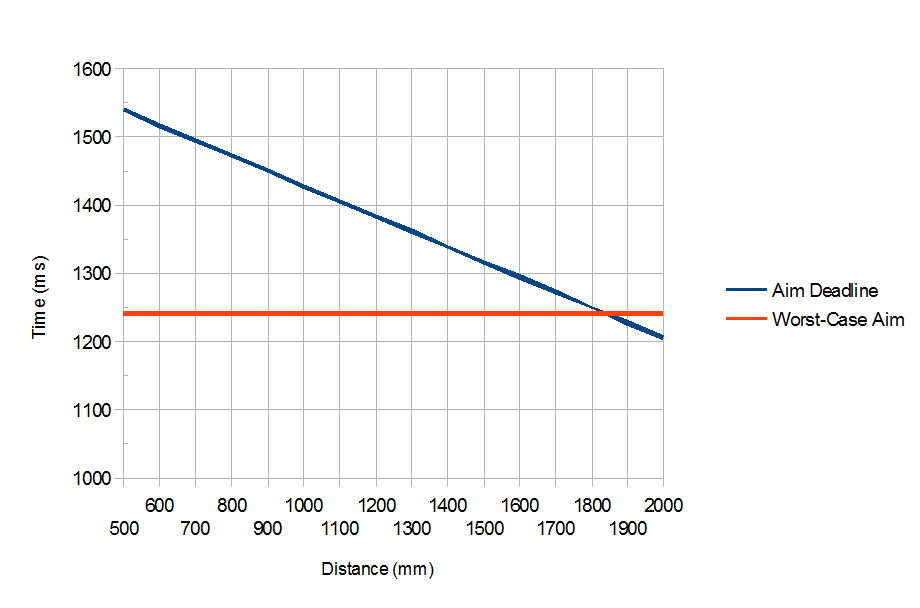
\includegraphics[scale=0.5]{img/deadline.png}
	\caption{Deadline for aim relative to distance}
	\label{fig:deadline}
\end{figure}
